%++++++++++++++++++++++++++++++++++++++++++++++++++++++++++
% This is the Slide for Leon Zhou's presentation
%++++++++++++++++++++++++++++++++++++++++++++++++++++++++++
\documentclass[slidestop,compress,mathserif,brown]{beamer}

%----------------------------------------------------------
% For source code list
%----------------------------------------------------------
\usepackage{listings}
\usepackage{verbatim}
\usepackage{CJK}
\usepackage{url}
\usepackage{amsmath,amssymb,amsfonts}
\usepackage{color,xcolor}
\usepackage{graphicx}
\usepackage{manfnt}

%----------------------------------------------------------
% font definition
%----------------------------------------------------------
\newcommand{\chuhao}{\fontsize{42pt}{\baselineskip}\selectfont}
\newcommand{\xiaochuhao}{\fontsize{36pt}{\baselineskip}\selectfont}
\newcommand{\yichu}{\fontsize{32pt}{\baselineskip}\selectfont} 
\newcommand{\yihao}{\fontsize{28pt}{\baselineskip}\selectfont}
\newcommand{\erhao}{\fontsize{21pt}{\baselineskip}\selectfont}
\newcommand{\xiaoerhao}{\fontsize{18pt}{\baselineskip}\selectfont}
\newcommand{\sanhao}{\fontsize{15.75pt}{\baselineskip}\selectfont}
\newcommand{\sihao}{\fontsize{14pt}{\baselineskip}\selectfont}
\newcommand{\xiaosihao}{\fontsize{12pt}{\baselineskip}\selectfont}
\newcommand{\wuhao}{\fontsize{10.5pt}{\baselineskip}\selectfont}
\newcommand{\xiaowuhao}{\fontsize{9pt}{\baselineskip}\selectfont}
\newcommand{\liuhao}{\fontsize{7.875pt}{\baselineskip}\selectfont}
\newcommand{\qihao}{\fontsize{5.25pt}{\baselineskip}\selectfont}

%----------------------------------------------------------
% Theme difinition
%----------------------------------------------------------
\usetheme{Antibes}
\usecolortheme{lily}

%----------------------------------------------------------
% Set title, author and date
%----------------------------------------------------------
\title{Bin Packing Heuristics}
\author{G14}
\date{\today}

%----------------------------------------------------------
%----------------------------------------------------------
\begin{document}
\begin{CJK}{UTF8}{kai}

%----------------------------------------------------------
% Style for source code list
%----------------------------------------------------------
\lstset{numbers=left, numberstyle=\tiny, basicstyle=\ttfamily\small,
keywordstyle=\color{blue!70},
commentstyle=\color{red!50!green!50!blue!50}, frame=shadowbox,
rulesepcolor=\color{red!20!green!20!blue!20},escapeinside=``,
xleftmargin=2em,xrightmargin=2em, aboveskip=1em}

%----------------------------------------------------------
% Title Page
%----------------------------------------------------------
\begin{frame}
\titlepage
\end{frame}

%----------------------------------------------------------
% Outline
%----------------------------------------------------------
\begin{frame}[shrink=1]
\frametitle{Outline}
\tableofcontents
\end{frame}

%----------------------------------------------------------
% Back ground introduction
%----------------------------------------------------------
\section{Back ground introduction}

\begin{frame}
\frametitle{Back Ground Introduction}
\begin{itemize}
	\item computational complexity theory, the bin packing problem is a combinatorial NP-hard problem. In it, objects of different volumes must be packed into a finite number of bins of capacity V in a way that minimizes the number of bins used.
	\item There are many variations of this problem, such as 2D packing, linear packing, packing by weight, packing by cost, and so on. They have many applications, such as filling up containers, loading trucks with weight capacity, creating file backup in removable media and technology mapping in Field-programmable gate array semiconductor chip design.
\end{itemize}
\end{frame}

\begin{frame}
\frametitle{Back Ground Introduction}
\begin{itemize}
	\item The bin packing problem can also be seen as a special case of the {\color{red}cutting stock problem}. When the number of bins is restricted to 1 and each item is characterised by both a volume and a value, the problem of maximising the value of items that can fit in the bin is known as the knapsack problem.
	\item Despite the fact that it is NP-hard, optimal solutions to very large instances can be produced with sophisticated algorithms. In addition, many heuristics have been developed.
\end{itemize}
\end{frame}

%----------------------------------------------------------
% Problems Introduction
%----------------------------------------------------------
\section{Packing problems}
\subsection{One-dimensional algorithms}
\begin{frame}
\frametitle{One-dimensional algorithms}
	\begin{itemize}
		\item Next Fit (NF) 
		\item First Fit (FF)
		\item Best Fit (BF) 
		\item Harmonic (HK) algorithm
		\item Next Fit-K (NFK)  
		\item	AFBK algorithm
		\item K-Bounded Best Fit (BBFK)  
		\item First Fit Decreasing (FFD)  
		\item Best Fit Decreasing (BFD)
	\end{itemize}
\end{frame}


\subsection{Other packing problems}
\begin{frame}
\frametitle{Other packing problems}
\begin{itemize}
	\item Packing in 2-dimensional containers:
	\begin{itemize}
		\item Circles in circle

		\begin{figure}
			\begin{center}
			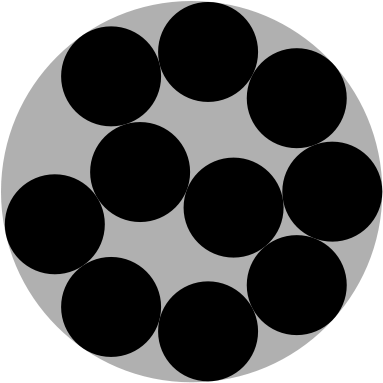
\includegraphics[height = 2cm]{figures/circleincircle.png}
			\end{center}
		\end{figure}

		\item Circles in square
	
		\begin{figure}
			\begin{center}
			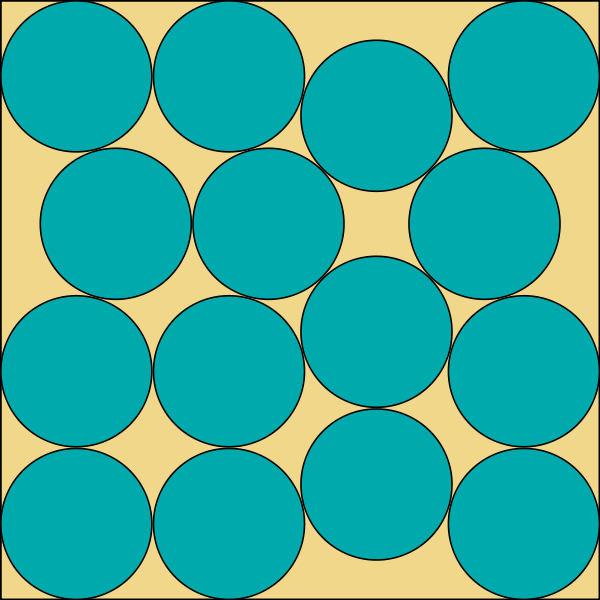
\includegraphics[height = 2cm]{figures/circleinsquare.png}
			\end{center}
		\end{figure}
	\end{itemize}
\end{itemize}
\end{frame}
		

\begin{frame}
\frametitle{Other packing problems}
\begin{itemize}
	\item Packing in 2-dimensional containers:
	\begin{itemize}
		\item Circles in isoscele right triangle(等腰直角三角形)

		\begin{figure}
			\begin{center}
			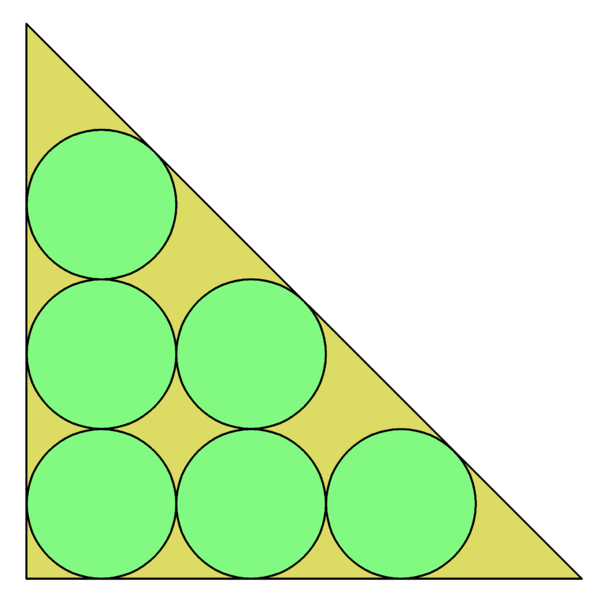
\includegraphics[height = 2cm]{figures/circleintri1.png}
			\end{center}
		\end{figure}

		\item Circles in equilateral triangle(等边三角形)
	
		\begin{figure}
			\begin{center}
			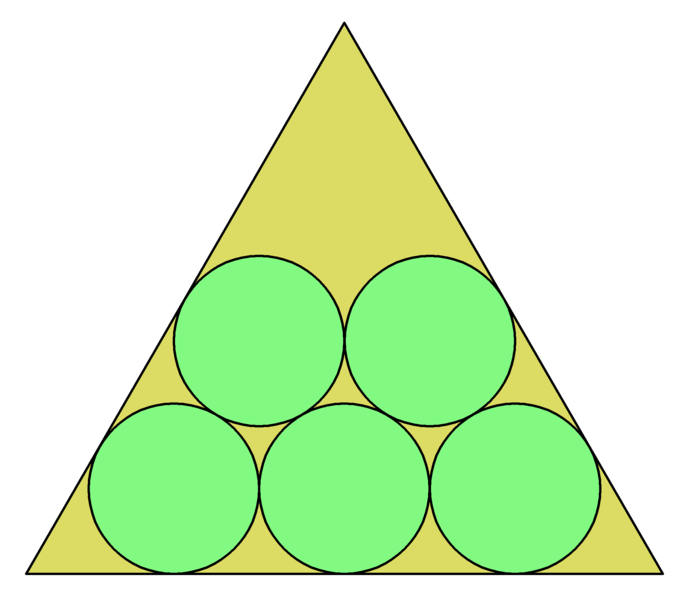
\includegraphics[height = 2cm]{figures/circleintri2.png}
			\end{center}
		\end{figure}
	\end{itemize}
\end{itemize}
\end{frame}


\begin{frame}
\frametitle{Other packing problems}
\begin{itemize}
	\item Packing in 2-dimensional containers:
	\begin{itemize}
		\item Squares in square

		\begin{figure}
			\begin{center}
			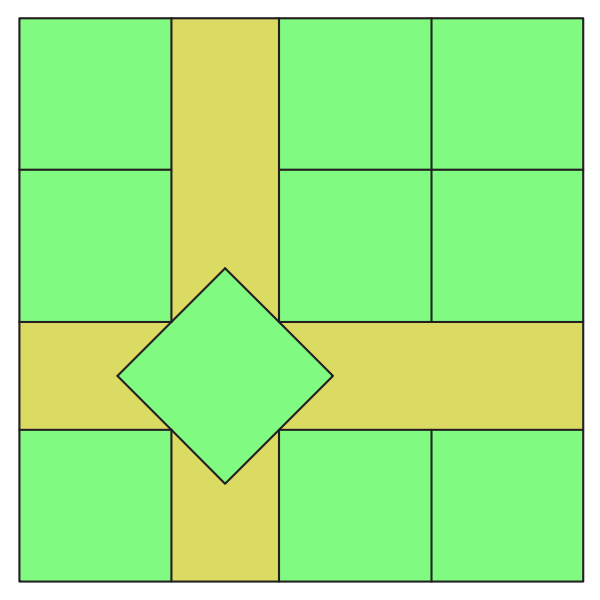
\includegraphics[height = 2cm]{figures/squinsqu.png}
			\end{center}
		\end{figure}

		\item Squares in circle
		\newline
		Pack n squares in the smallest possible circle.
	\end{itemize}
\end{itemize}
\end{frame}

\begin{frame}
\frametitle{Other packing problems}
\begin{itemize}
	\item Packing in 3-dimensional containers:
 	\begin{itemize}
 		\item Spheres into a Euclidean ball
		\item Spheres in a cuboid
 	\end{itemize}
	\item Packing of irregular objects
\end{itemize}
\end{frame}

%----------------------------------------------------------
% Test of FF NF BF FFD
 %----------------------------------------------------------
\section{Implementation}
\subsection{Main idea}
\begin{frame}
\frametitle{Main idea}
\begin{itemize}
	\item NF:
	\begin{itemize}
		\item Time complexity: $O(n)$
	\end{itemize}
	\item FF:
	\begin{itemize}
		\item We use the most naive way, check the bins from the very beginning until find one bin fits.
		\item Time complexity: $O(n^2)$
	\end{itemize}
	\item BF:
	\begin{itemize}
		\item We use a binary search tree to store the free capacity of bins, and find the bin to store new element from the tree. The full bin are not in the search tree.
		\item Time complexity: $O(nlogn)$
	\end{itemize}
	\item FFD:
	\begin{itemize}
		\item FFD is the only off-line algorithm in these four. First sort the inputs, then apply FF to them.
		\item Time complexity: $O(n^2)$
	\end{itemize}
\end{itemize}
\end{frame}

\subsection{Test of different input size}
\begin{frame}
\frametitle{Test of different input size}
\begin{figure}
	\begin{center}
	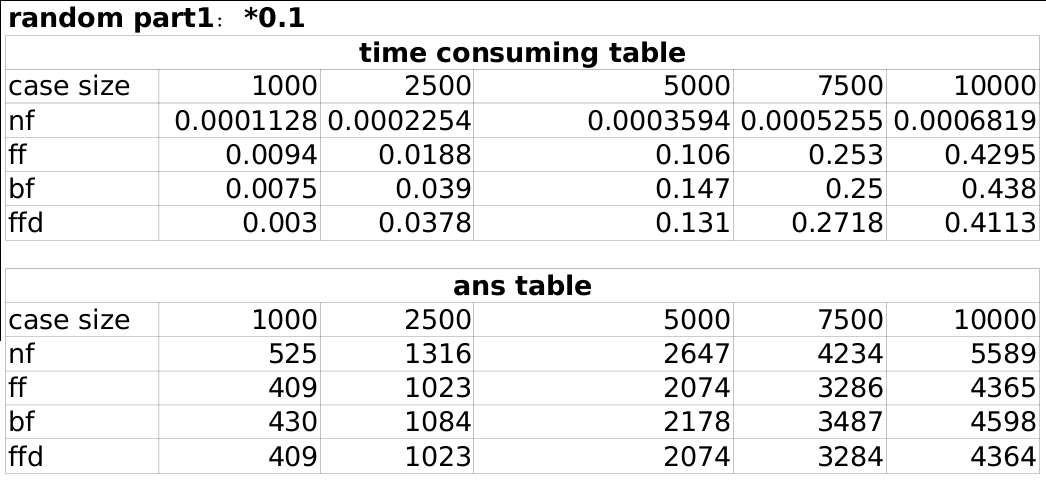
\includegraphics[height = 3cm]{figures/1.png}
	\end{center}
	\begin{center}
	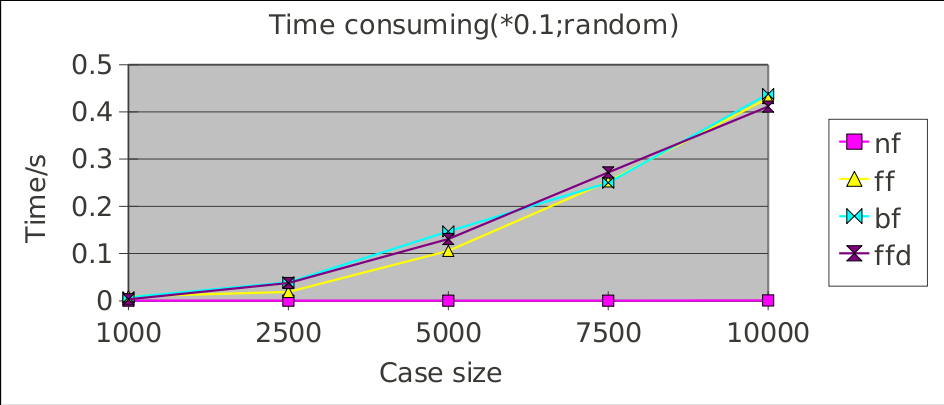
\includegraphics[height = 2cm]{figures/4.png}\quad
	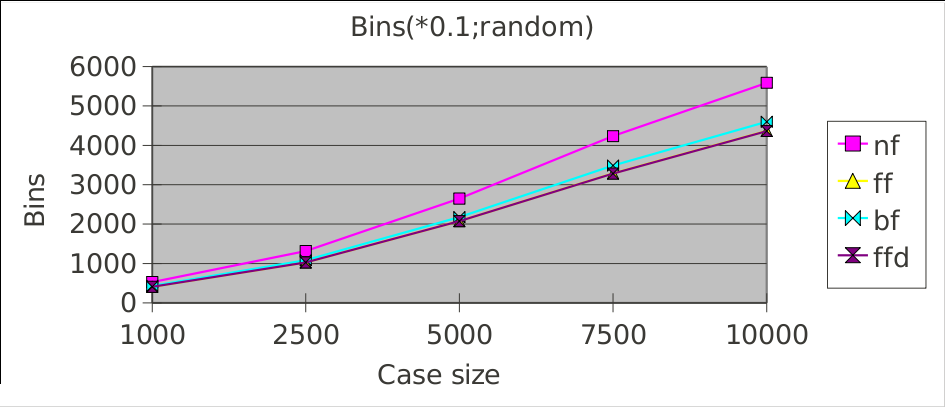
\includegraphics[height = 2cm]{figures/7.png}
	\end{center}
\end{figure}
\end{frame}

\begin{frame}
\frametitle{Test of different input size}
\begin{figure}
	\begin{center}
	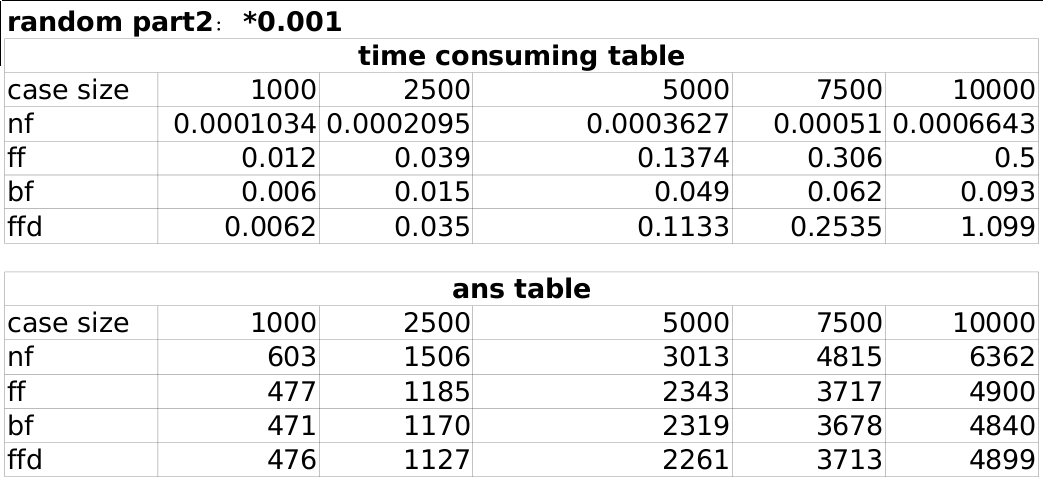
\includegraphics[height = 3cm]{figures/2.png}
	\end{center}
	\begin{center}
	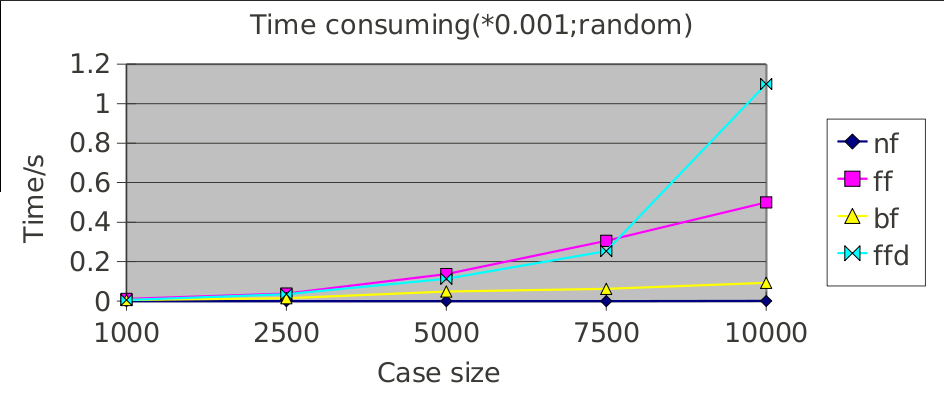
\includegraphics[height = 2cm]{figures/5.png}\quad
	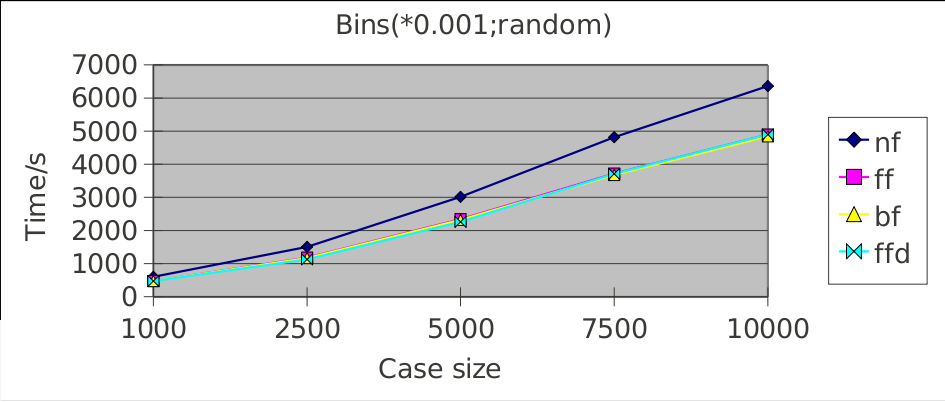
\includegraphics[height = 2cm]{figures/8.png}
	\end{center}
\end{figure}
\end{frame}

\subsection{Test of different ordered input}
\begin{frame}
\frametitle{Test of different ordered input}
\begin{figure}
	\begin{center}
	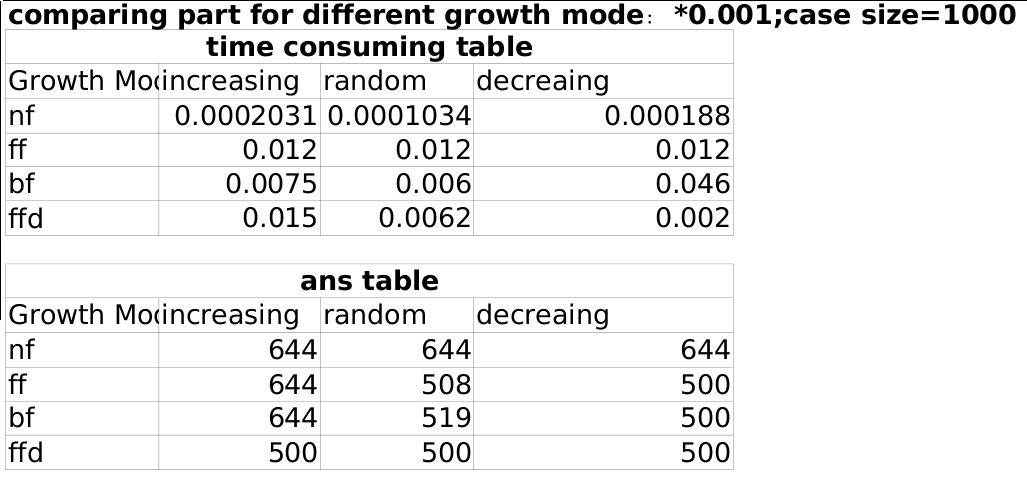
\includegraphics[height = 3cm]{figures/3.png}
	\end{center}
	\begin{center}
	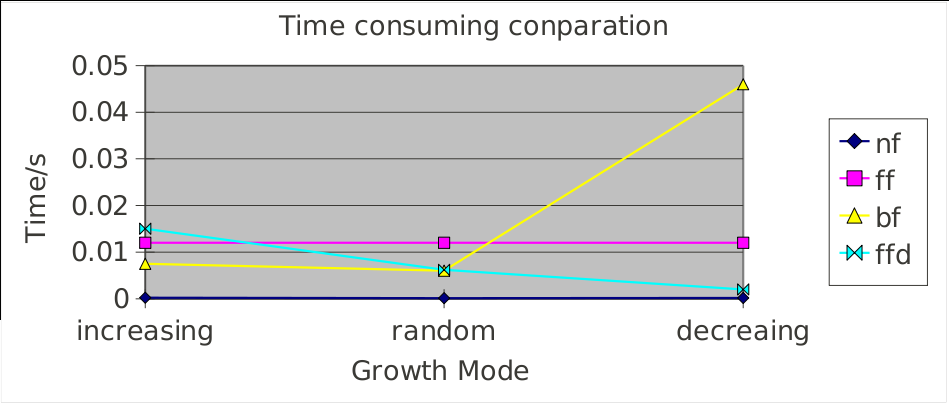
\includegraphics[height = 2cm]{figures/6.png}\quad
	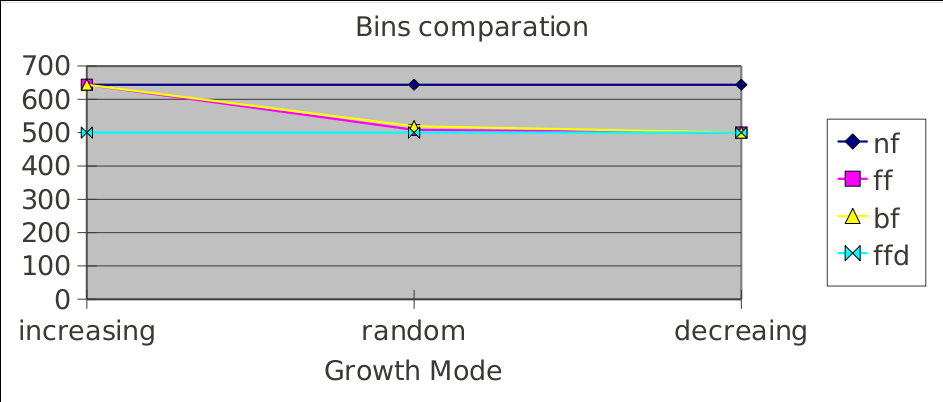
\includegraphics[height = 2cm]{figures/9.png}
	\end{center}
\end{figure}
\end{frame}



%----------------------------------------------------------
% Cutting stock problem
%----------------------------------------------------------
\section{Cutting stock problem}
\subsection{First Fit}
\begin{frame}
\frametitle{First Fit in Cutting stock}
In the first fit algorithm, the allocator keeps a list of free blocks (known as the free list) and, on receiving a request for memory, scans along the list for the first block that is large enough to satisfy the request. If the chosen block is significantly larger than that requested, then it is usually split, and the remainder added to the list as another free block.
\newline
The first fit algorithm performs reasonably well, as it ensures that allocations are quick. When recycling free blocks, there is a choice as to where to add the blocks to the free list -- effectively in what order the free list is kept:
\end{frame}

\subsection{Best Fit}
\begin{frame}
\frametitle{Best Fit in Cutting stock}
Increasing size
\newline
This is equivalent to the best fit algorithm, in that the free block with the "tightest fit" is always chosen. The fit is usually sufficiently tight that the remainder of the block is unusably small.
\end{frame}

\subsection{Worst Fit}
\frametitle{Worst Fit in Cutting stock}
\begin{frame}
Decreasing size
\newline
This is equivalent to the worst fit algorithm. The first block on the free list will always be large enough, if a large enough block is available. This approach encourages external fragmentation, but allocation is very fast.
\end{frame}

%----------------------------------------------------------
% something more
%----------------------------------------------------------
\section{something more}
\begin{frame}
\begin{itemize}
	\item test the new plugin
	\item I think is very useful for me to use \LaTeX{}
	\item The curent version is \LaTeXe.
\end{itemize}
\end{frame}
\end{CJK}
\end{document}
